\documentclass{sig-alternate}

% UTF8 support
\usepackage[utf8x]{inputenc}


\usepackage{hyperref}
\usepackage{epsf,graphicx}
\graphicspath{{figures/}}
\usepackage{subfigure}
\usepackage[colorinlistoftodos]{todonotes}

\newcommand{\eg}{{\textit{e.g.~}}}
\newcommand{\etal}{{\textit{et al.~}}}
\newcommand{\ie}{{\textit{i.e.~}}}

%
% --- Author Metadata here ---
\conferenceinfo{10th ACM/IEEE International Conference on Human-Robot Interaction}{2015 Portland, USA}
%\CopyrightYear{2007} % Allows default copyright year (20XX) to be over-ridden - IF NEED BE.
%\crdata{0-12345-67-8/90/01}  % Allows default copyright data (0-89791-88-6/97/05) to be over-ridden - IF NEED BE.
% --- End of Author Metadata ---

%(DH) is it too soon to claim learning by teaching benefits in the title...? 
%(DH) the paper is not about "learning handwriting", it's about the robot.
\title{\LARGE \bf
``Those who can't do, teach'': a Teachable Robotic Agent for Children Learning Handwriting
}


%%% HRI 2015 -> double-blind review process

% \numberofauthors{3} 
% \author{
% \alignauthor
% Deanna Hood\\
% Séverin Lemaignan\\
% Pierre Dillenbourg\\
%    \affaddr{Computer-Human Interaction in Learning and Instruction Laboratory (CHILI)}\\
%    \affaddr{École Polytechnique Fédérale\\ de Lausanne (EPFL)}\\
%    \affaddr{CH-1015 Lausanne, Switzerland}\\
%    \email{firstname.lastname@epfl.ch}
% \alignauthor
% Rafael Garcia\\
%    \affaddr{Computer Vision and Robotics Group (ViCOROB)}\\
%    \affaddr{University of Girona}\\
%    \affaddr{Girona, Spain}
% }

%(DH) my EPFL email address won't work for much longer....


\begin{document}



\maketitle

%%%%%%%%%%%%%%%%%%%%%%%%%%%%%%%%%%%%%%%%%%%%%%%%%%%%%%%%%%%%%%%%%%%%%%%%%%%%%%%%
\begin{abstract}

%Despite the social motivation for the use of a teachable agent for the
%engagement and support of children with handwriting difficulties, to date no
%such technology is known to have been developed. 

%(DH) abstract probably too long...
%(DH) do we have to be specific somewhere about what stage of handwriting we're targeting..?

Presented is a teachable humanoid agent in the context of handwriting skills
acquisition. It is hypothesised that such a system could not just engage an
unmotivated student, but could also present the opportunity for children to
experience the typical benefits experienced during human-led handwriting
interventions, such as motor mimicry. This system allows for exploring the
potential for the \emph{learning by teaching} paradigm to be employed in the
interaction, so as to stimulate meta-cognition, empathy and increased
self-esteem in the child user. 

By leveraging simulated handwriting on a synchronised tablet display, a Nao
humanoid robot with limited fine motor capabilities has been configured as a
suitably embodied handwriting partner. Shape models derived from principal
component analysis of a dataset of letter trajectories are generated and allow
the robot to draw purposefully deformed letters. Learning how to write
characters well is then achieved by incorporating feedback from user
demonstrations, which allows the system to learn the optimal parameters for the
appropriate shape models. 

An in situ study has been conducted with primary school classes to obtain
insight into children's use of the novel system. 
%The technical components of the system have been validated, in that children 
Children aged 6-8 were successfully 1) led to believe that the robot was
actually writing on the tablet, and 2) able to improve the robot's writing to a
level which they were satisfied with. Furthermore, the system represents a
significant step towards an innovative use for robotics which addresses a
widespread and socially meaningful challenge in education, and provides context
for robotics in education beyond the well-explored use of teaching coding- and
robotics-related subjects.

\end{abstract}


%%%%%%%%%%%%%%%%%%%%%%%%%%%%%%%%%%%%%%%%%%%%%%%%%%%%%%%%%%%%%%%%%%%%%%%%%%%%%%%%
\section{INTRODUCTION}

Handwriting difficulties in children at an early age often negatively affect
the academic performance of the students \cite{Christensen2005}, in addition to
their self-esteem being adversely affected \cite{Malloy1995}, causing them to
shy away from expressing what they know \cite{Medwell2008}.
%A conclusion drawn
%in \cite{Hoy2011} is that any handwriting intervention studies considered in the
%systematic review which involved fewer than two practice sessions per week and
%fewer than a total of 20 practice sessions, including homework, were found to
%demonstrate ineffective results. This highlights the necessity to engage
%students in an interaction that will be sustainable over the long-term. 

Successful interventions for children with handwriting difficulties involve the
student in many sessions where they are engaged in physically practising the
skill \cite{Hoy2011}. However, the link between handwriting difficulties and low
self-efficacy \cite{Engel-Yeger2009} results in children who are unmotivated to
participate in such sessions, potentially leading to a developmental arrest in
the acquisition of the skill. 

%Engel-Yeger, Nagauker-Yanuv and Rosenblum \cite{Engel-Yeger2009} have shown the
%link between handwriting difficulties and low self-efficacy, the belief in
%one's capabilities to complete a task. Bandura \cite{Bandura1990} maintains
%that self-efficacy constitutes the basis for the choice of whether or not to
%attempt a task. Indeed, third graders receiving intervention for their
%handwriting skills in \cite{Berninger1997} spoke of how they avoid writing
%because of how it is illegible to others. This mindset of believing that one is
%unable to write may lead to a developmental arrest in the acquisition of this
%skill, which may make intervention more difficult in the future. Consequently,
%it is of importance to engage students in activities in which their
%self-efficacy and self-motivation is restored.

The \emph{learning by teaching} paradigm, which engages the target student in
the act of teaching another, has been shown to produce motivational,
meta-cognitive, and educational benefits in a range of disciplines
\cite{Rohrbeck2003}. An application which is yet to be explored, however, is the
application of learning by teaching to handwriting intervention. One reason why
this has not been investigated to date is that in order to engage a child in the
learning by teaching paradigm, there must be an appropriately unskilled peer for
them to tutor. In the context where the target child is the lowest performer in
their class, this may be a constraint. In some cases it may be appropriate for a
peer or teacher to simulate a na\"ive learner for the target child to teach,
however for an activity where one's skill level is visually evident - as is the
case in handwriting - this acting is likely to be eventually detected. As such,
there is motivation for the use of a teachable agent which can be configured for
a variety of skill levels, and for which children do not have preconceptions
about its handwriting ability.

Presented is the development of the first known learning agent which is capable
of artificially making mistakes typical of children learning handwriting, and
correcting them with external feedback. Such a system therefore exhibits the potential
to engage children in the learning by teaching paradigm in the context of
handwriting. 

There are three main points which have motivated the use of a robot as the
teachable agent in the presented interaction:

\begin{enumerate}
    \item the engagement and ``protégé effect'' elicited by teaching an embodied
        agent is anticipated to be stronger than that associated with a
        tablet-based application, which children are increasingly recognising as
        disposable technology,

    \item observing a teachable agent respond to what it has been taught
        \cite{Okita2006} is a significant step in the learning by teaching
        paradigm, and therefore it may be significant for the agent to respond
        with a writing \emph{process}, rather than simply a product, and

    \item the potential for motor mimicry to yield significant improvements in
        handwriting interventions \cite{Berninger1997} further supports the case
        for investigating the use of a humanoid robot capable of physically
        demonstrating handwriting trajectories to its child learning partner.
\end{enumerate}

Consequently, the learning agent developed has been embodied in a commercially
affordable Nao humanoid robot. Its writing capabilities have been implemented by
leveraging synchronisation with a tablet display to simulate fine motor skills
otherwise infeasible for the robot. 

Section \ref{sec:learningAlgorithm} presents the novel work in the area of
artificial intelligence to develop a learning algorithm suitable for a learning
agent in the context of handwriting.  Section \ref{sec:robotWriting} details the
extension of this algorithm to an embodied robotic learning agent, including the
novel approach for achieving simulated fine motor skills on commercially
affordable humanoid robots.  Section \ref{sec:experiment} explores the novel
contributions made to the study of human-robot interaction, in discussing the
use of the system with primary school children and its potential as a tool for
addressing wider pedagogical research questions in education. 



%%%%%%%%%%%%%%%%%%%%%%%%%%%%%%%%%%%%%%%%%%%%%%%%%%%%%%%%%%%%%%%%%%%%%%%%%%%%%%%%
\section{A Learning Agent in the Context of Handwriting} \label{sec:learningAlgorithm}

Because of the objective to use an artificial intelligence algorithm in a
reinforcement learning framework, a parameterisation of letters and their
deformities has been sought. Depending on the parameters input to the letter
models, different quality shapes can be generated. The system can therefore be
configured to improve its writing by modifying the parameters used to generate
the letters, based on feedback from the reinforcement learning partner. To this
end, a method which can generate a model from real-world data has been employed
in order to capture realistic variations in letters. 

\subsection{Shape Modelling of Letters} \label{sec:writingGeneration}

One approach for a shape model which can appropriately represent realistic
variations in shapes with changes to its parameters is statistical shape
modelling. Statistical shape modelling is an application of principle component
analysis (PCA), where a linear transform which de-correlates data vectors is
found \cite{Stegmann2002} and allows for dimensionality reduction. 

PCA has been performed on a set of letter paths captured from a digital pen,
using the UJI Pen Characters 2 dataset \cite{Llorens2008} with 120 instances of
each letter (2 repetitions from 60 adult users). While it may be appropriate to
identify the location of the most salient features of the shapes in future work,
the features are currently taken as $n$ uniformly spaced points along the shape
path as salient features are not guaranteed from children's handwriting. The
points are arranged into an observation vector presented in (\ref{eq:obsVec}),
where $x_i$ and $y_i$ represent the coordinates of each of the points along the
path.

\begin{equation}\label{eq:obsVec}
{\bf x} = [x_1, x_2, \ldots, x_n, y_1, y_2, \ldots, y_n]^T
\end{equation}

In this work, the observation shapes are normalized such that they have a shape
centre of ${\bf 0}$ and a unit maximum dimension. 

The projection from the original $2n$-dimensional feature space $(n=70)$ to an
$N$-dimensional space is found as in (\ref{eq:projection}), where ${\bf p}$
contains the coordinates in the $N$ dimensional space with ${\bf 0}$-origin,
calculated as in (\ref{eq:paramCalc}). The $2n\times N$ matrix ${\bf \Phi }$ is
an orthogonal matrix composed of the eigenvectors ${\bf v}_i$ corresponding to
the largest $N$ eigenvalues ($\lambda_i$) of the covariance matrix of the
observations, as shown in (\ref{eq:transformCalc}) \cite{Stegmann2002}. As such,
each shape may be approximated by the mean shape plus a sum of the top $N$
eigenvectors, weighted by the parameter vector $p$. 

\begin{equation}\label{eq:projection}
{\bf \tilde{x}=\bar{x}+\Phi p}
\end{equation}
\begin{equation}\label{eq:paramCalc}
{\bf p} ={\bf \Phi}^T ({\bf {x}-\bar{x}})
\end{equation}
\begin{equation}\label{eq:transformCalc}
{\bf \Phi} = [{\bf v}_1, {\bf v}_2, \ldots, {\bf v}_N]^T
\end{equation}

If there is correlation between the points in the observations, there will be
eigenvalues of the covariance matrix which are close to zero. As such, removing
the associated eigenvectors from ${\bf \Phi}$ allows for dimensionality
reduction with minimal impact. Indeed, the amount of variance in the dataset
that is explained by each eigenvector ${\bf v}_i$ is $\sqrt{\lambda_i}$, and
therefore the proportion of the variance explained by each dimension/eigenvector
is as shown in (\ref{eq:proportionVar}).

\begin{equation}\label{eq:proportionVar}
\%var_i = \frac{\sqrt{\lambda_i}}{\sum_{i=1}^{N}\sqrt{\lambda_i}}\times 100\%
\end{equation}

For the dataset presented in Figure \ref{fig:deviations_sPrint}, the
eigenvectors associated with the 5 largest eigenvalues explain 90.0\% of the
variance in the dataset, illustrating the capability of the statistical shape
modelling approach to produce compact parameterisation of shapes. 

Clusters within paths of a particular letter have been identified using K-means
clustering to group different styles of writing the letter (\emph{allographs}),
such that the parameters in the resulting model are only representative of the
specific allograph of the letter in the dataset. 
% * <deanna.m.hood@gmail.com> 2014-09-03T13:05:23.576Z:
%
% in the end this was pointless so maybe not worth mentioning
%
PCA has been performed on all of the paths of a particular allograph in the
dataset at a time, to reduce the $2n$ dimensional space to one of a desired
number of dimensions.

(\ref{eq:projection}) may be used
to generate new shapes based on the parameters ${\bf p}$ which are used: ${\bf
p}={\bf 0}$ will yield the mean shape, and variations to each of the $N$ values
in ${\bf p}$ will cause a change in the shape represented by the corresponding
eigenvector (Figure \ref{fig:deviations_sPrint}). 

\begin{figure}[thpb]
\centering
\subfigure{
\raisebox{-0.5\height}{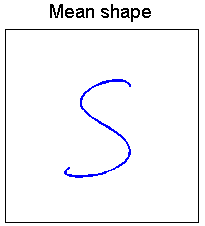
\includegraphics[width=0.05\textwidth]{figures/sPrint_mean.png}
}}
\subfigure{
\raisebox{-0.5\height}{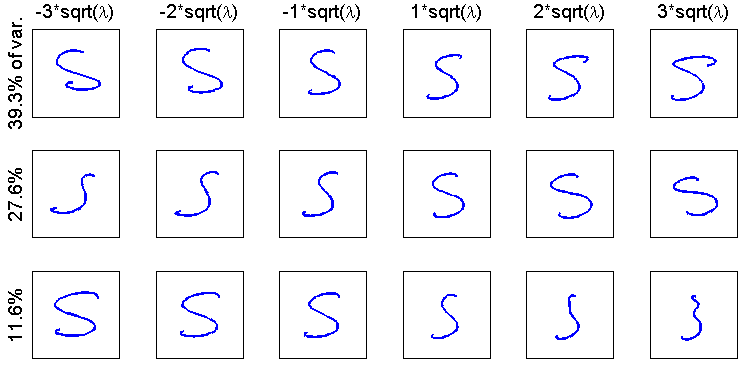
\includegraphics[width=0.35\textwidth]{figures/sPrint_top3.png}
}}
\caption[The mean shape and the effect of varying the first three parameters of
the shape model derived from PCA from the dataset of print `s'
shapes.]{\label{fig:deviations_sPrint}The mean shape (left) and the effect
    (right) of varying the first three parameters (each row) of a shape model.
    The presented model has been derived from PCA on the first cluster of `s'
    shapes, interpreted as the print allograph. The extent to which each
parameter is varied is dependent on the eigenvector $\lambda$ corresponding to
the parameter's eigenvector. The percentage of the total variance in the dataset
explained by each parameter is shown to the left of the corresponding row. }

\end{figure}

Interestingly, although the parameters are the result of an \emph{unsupervised}
statistical shape analysis, they still represent variations which could have
been intuitively identified by a manual parameterisation. For example, for the
model shown in Figure \ref{fig:deviations_sPrint}, the parameters may represent
the width of the top half of the letter compared to the bottom half, the width
of the overall shape, etc. Consequently, the shape modelling process has
produced the desired outcomes of parameterising the shapes in ways which are
able to be used to deform them meaningfully.


\subsection{Generating Poor Letters}

After determining the appropriate number of dimensions ($N$) for the shape
models, new letters can be generated by varying the parameter values in this
$N$-dimensional space in accordance with (\ref{eq:projection}). By choosing
parameter values which lie within the observed range in the dataset, it is
possible to produce letters which are more likely to be reasonable looking.
When the parameter values are outside of the range observed in the dataset, they
are less likely to represent shapes from the dataset of reasonable,
adult-written letters, and as a result are more likely to represent poor shapes.
Figure \ref{fig:sampleLetters} illustrates sample letters generated from the
models of `e' and `g' - made from 120 observations each, with 70 sample points -
by selecting random values for the first 5 parameters from a distribution with
standard deviation of $3\sqrt\lambda_i$ rather than the $\sqrt\lambda_i$
standard deviation observed in the dataset.

\begin{figure}[thpb]
\centering
\subfigure{\raisebox{-0.5\height}{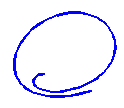
\includegraphics[height=0.08\textwidth]{figures/e1.png}}}
\subfigure{\raisebox{-0.5\height}{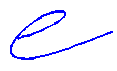
\includegraphics[height=0.05\textwidth]{figures/e4.png}}}
\subfigure{\raisebox{-0.5\height}{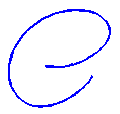
\includegraphics[height=0.08\textwidth]{figures/e3.png}}}
\subfigure{\raisebox{-0.5\height}{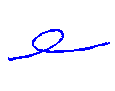
\includegraphics[height=0.08\textwidth]{figures/e5.png}}}\\
\subfigure{\raisebox{-0.5\height}{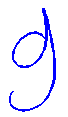
\includegraphics[height=0.12\textwidth]{figures/g1.png}}}
\subfigure{\raisebox{-0.5\height}{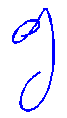
\includegraphics[height=0.12\textwidth]{figures/g3.png}}}
\subfigure{\raisebox{-0.5\height}{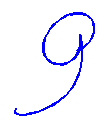
\includegraphics[height=0.12\textwidth]{figures/g4.png}}}
\subfigure{\raisebox{-0.5\height}{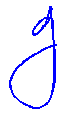
\includegraphics[height=0.12\textwidth]{figures/g5.png}}}
\caption[Sample letters generated from the PCA shape model on 120 `e' and `g'
paths.]{\label{fig:sampleLetters}Sample letters generated from the PCA shape
model on 120 `e' (top) and `g' paths (bottom), generated randomly from
parameters with $3\times$ the standard deviation observed in the dataset.}

\end{figure}

In \cite{Chandra2013}, it was found that children aged 4-6 years participating
in a handwriting peer tutoring pilot study most often made mistakes classified
as inappropriate \emph{internal proportions} or \emph{global deformations}. It
would be reasonable to consider the shapes in Figure \ref{fig:sampleLetters} in
the same general categories. Using a database of children's letters when
available may yield potential for parameterising other mistakes made by
children, such as merging strokes or decomposing a shape into multiple subparts
inappropriately. Nevertheless, sufficient capabilities for the shape model to
generate `poor' letters which are appropriate for simulating a na\"ive learning
in the context of handwriting have been demonstrated, using the shape model
generated with PCA from a dataset of only adults' writing.


\subsection{Responding to Feedback}

It was shown in Section \ref{sec:writingGeneration} how the statistical shape
model of a particular letter may convert a set of parameters into a generated
letter of the same allograph. Similarly, the model may also be used to convert a
letter into its parameters, given the model. The parameters of user-drawn
letters may therefore be used in order to incorporate the capabilities for the
learning algorithm to adapt to the user's feedback via demonstration.

The statistical shape model may be used to determine the parameters of a
demonstration shape by projecting the features of the observed shape into the
lower-dimensional space determined by the model. Mathematically, given a
demonstration ${\bf x}_{demo}$, the associated parameters may be determined as in
(\ref{eq:param}).

\begin{equation}\label{eq:param}
{\bf p}_{demo} ={\bf \Phi}^T ({\bf{x}_{demo}-\bar{x}})
\end{equation}

The parameters which are determined for a shape in (\ref{eq:param}) will not
reconstruct the shape exactly if $N<2n$, but rather will reconstruct the closest
point in the $N$-dimensional space which the eigenvectors span. $N=10$ has been
used for the work presented.

For the statistical shape model employed by the system, the method for
responding to user demonstrations is to move the learning algorithm's parameters
towards those of the demonstration to some extent. In the results presented in
this work, \[{\bf p}^{(k+1)} = {\bf p}^{(k)} + ({\bf p}_{demo}-{\bf
p}^{(k)})\times\alpha\] has been used, where ${\bf p}$ is the parameter vector
at time step $k$, and $\alpha$ is the learning rate, between 0 and 1.  It is
possible that parameters ${\bf p}^{(k)}$ and ${\bf p}_{demo}$, which
individually yield acceptable shapes, may produce parameters ${\bf p}^{(k+1)}$
which yield an unacceptable shape. The proposed method for adapting to user
demonstration would not get stuck at such poor shapes, however: with further
demonstrations of the same letter, the system would eventually approach it. As a
result, this event would not limit the interaction proposed in Section
\ref{sec:experiment}, but it may influence the user's perception of the learning
agent. It remains to be seen if it is necessary to avoid such an event
mathematically.

Figure \ref{fig:demonstrationShapes2} illustrates the response of the system to
demonstrations from a child for the letter `u' using a learning rate of
$\alpha=1/2$. 

\begin{figure}[thpb]
    \centering
    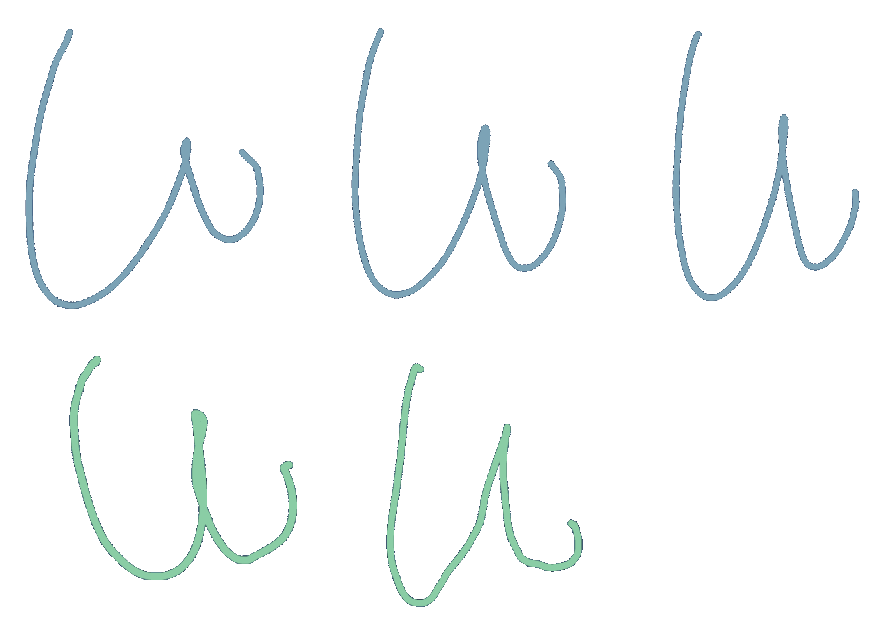
\includegraphics[width=0.3\textwidth]{figures/u_kids.png}
    \caption{\label{fig:demonstrationShapes2}Example of the learning algorithm
    responding to user demonstration of shapes for the letter `u.'}
\end{figure}

% * <deanna.m.hood@gmail.com> 2014-09-04T09:19:16.057Z:
%
% improve img
%



%%%%%%%%%%%%%%%%%%%%%%%%%%%%%%%%%%%%%%%%%%%%%%%%%%%%%%%%%%%%%%%%%%%%%%%%%%%%%%%%
\section{An Embodied Handwriting Learning Agent with the Nao Humanoid Robot} \label{sec:robotWriting}

In order to develop a teachable agent that is appropriate for engaging a child
through the learning by teaching paradigm, 
%- that is, that it is an embodied agent, capable of eliciting motor mimicry,
%and capable of causing its teacher to reflect on the process that has been used
%to respond to handwriting feedback -
capabilities for the robot to engage in handwriting have been established.

The Nao humanoid robot, which has been developed by Aldebaran-Robotics and
designed purposely to look approachable \cite{Gouaillier2008}, has been used for
this work. It is a commercially affordable biped robot, 58cm tall, with 25
degrees of freedom, two cameras, speech capabilities and the ability to
autonomously execute a range of tasks.

%Because of the challenges in getting the Nao to write trajectories smoothly
%because of its inherent ability to only reach discrete points in space, 
A fine level of control over what the robot is writing is necessary in the
proposed application of a learning agent in the context of handwriting. Because
of the limited fine motor skills possible with such an affordable robot, in
addition to the absence of force feedback and other technical necessities, the
Nao has been configured to use simulated handwriting with a synchronised tablet
to achieve this level of control. The necessary components of implementing the
proposed teachable robotic agent are, therefore:

\begin{enumerate}
    \item developing capabilities for the robot to trace handwriting, 

    \item synchronising the robot's movements with the display of the writing on a
        tablet so that it seems that the robot is causing the handwriting to
        display because of its actions, and

    \item integrating the writing behaviour with the handwriting learning
        algorithm presented in Section \ref{sec:learningAlgorithm} to create a
        \emph{learning by teaching} interaction with the agent. 
\end{enumerate}

These steps are presented in the sections which follow.

\subsection{Robot Trajectory Following}

Using simulated handwriting provides an opportunity for the robot's writing to
appear smoother than would be achievable with a writing instrument. However, the
robot's motions must still sufficiently match the displayed trajectory in order
capture the engagement of the child user in the action.

Aldebaran's NaoQi API has been used for the inverse kinematics of the trajectory
following. The Robot Operating System (ROS)\footnote{The ROS stack for Nao is
available at: \url{http://wiki.ros.org/nao_robot}} has been used for integration
of the Nao with external reference frames using the $tf$ transformation library
\cite{Foote2013}, such as the tablet's location.

When using simulated handwriting, it is no longer necessary that the robot
engages in the typical style of handwriting with a writing instrument at a desk.
By instead having the robot point at a vertical writing surface to cause the
trajectory to appear (as in Figure \ref{fig:naoWriting}), several advantages are
presented:

\begin{itemize}

    \item The working space of the robot increases, both in the technical sense
        and the interaction sense: someone can, in theory, show the tablet to
        the robot from across the room and have it still respond, without
        needing the tablet to be within arm's reach.

    \item Concerns about whether or not the child would start mimicking the
        robot's incorrect (inhuman) writing style are mitigated. % * <deanna.m.hood@gmail.com> 2014-09-04T09:59:44.707Z:
%
% is this point significant enough?
%

    \item Perhaps most significantly, the accuracy of the matching of the
        robot's motion with the trajectory displayed on the tablet is not as
        critical, because the finger is not expected to touch the tablet exactly
        at the trajectory point, in contrast to the pen tip.
        % This means that orientation degrees of freedom can be freed without significant adverse effects.

\end{itemize}

\begin{figure}[thpb]
     \begin{center}
        %\subfigure{
        %    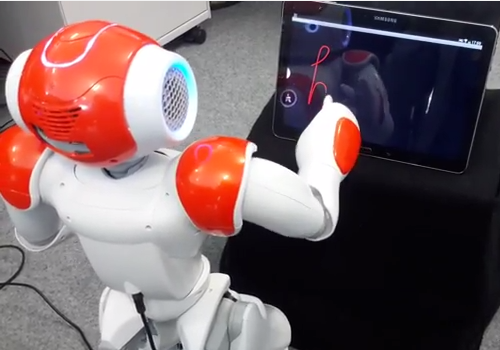
\includegraphics[width=0.4\textwidth]{figures/naoWriting1.png}
        %}%
        \subfigure{
            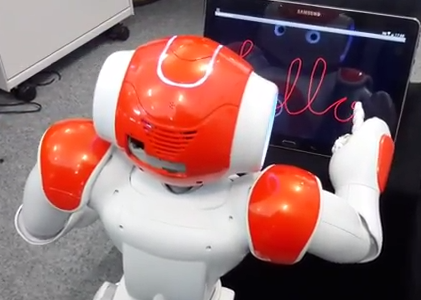
\includegraphics[width=0.3\textwidth]{figures/naoWriting2.png}
        }%
%
    \end{center}
    \caption{A demonstration of the robot simulating the writing of a word
        with its finger. The motion of the robot is synchronised with the display of the tablet, communicating over ROS.
     }%

   \label{fig:naoWriting}
\end{figure}

Therefore, the system presented utilises the context where the robot is
simulating handwriting by pointing at the tablet\footnote{Teachers interviewed
for their feedback on the system advised that children are asked to draw letters
in the air in a similar manner as part of their handwriting education.}. Because
motion planning is performed with respect to the hand of the robot, rather than
its fingertip, the one or two of the orientation degrees of freedom of the hand
are fixed to keep the finger approximately perpendicular to the writing surface,
depending on the desired accuracy. The remaining free orientation(s), coupled
with the whole-body motion control available, allow for a sufficient working
space for writing on the entire tablet.

\subsection{Synchronisation with the Tablet Trajectory Display}\label{sec:tabletSynch}

After getting the robot to trace writing trajectories, the next step towards
simulated handwriting is getting the trajectories of the robot's `writing' to
display on an Android tablet. 

ROS has been used for the communication between the devices used in the system,
including the Android tablet\footnote{For more information about ROS on Android
devices see \url{http://wiki.ros.org/android}}. As a result, aspects of the
networking between the tablet and the robot, such as the overheads associated
with connections, ports, message formats, etc. have been simplified. 

An Android application has been developed to receive the trajectory message over
a ROS topic and add each point of the trajectory one by one as a frame of an
animation. Synchronisation between the tablet and the robot has been achieved by:

\begin{itemize}

    \item sending a requested start time accompanying the trajectory, which is
        sufficiently in the future, to account for varying transmission delays
        to the nodes on different devices,

    \item synchronising all clocks with NTP servers such that the ROS time used
        for responding to the requested start time is the same at all nodes,

    \item reducing the number of points along the trajectory passed to the
        robot's motion planner, to improve timing accuracy, and

    \item not running computationally expensive tasks on the robot (such as
        camera publishing) while it is writing, as this interferes with the
        requested timings between points. 

\end{itemize}

To instruct the robot where to write, the robot has been configured to detect a
particular fiducial marker, a \emph{chilitag}\footnote{See
\url{https://github.com/chili-epfl/ros_markers} for more information on the
fiducial markers used.}, with the camera located in its head and use that as the
origin of the writing surface (Figure \ref{fig:tabletDetection}). When used in
an interaction with a child, this allows the user to move the tablet as required
for the interaction. As publishing the robot's camera has been identified as a
computationally expensive task which can disrupt the robot's timing of
synchronised writing, it is only done when the robot is not writing, and the
tablet is assumed to be stationary during the writing process.

\begin{figure}[htpb]
    \centering
    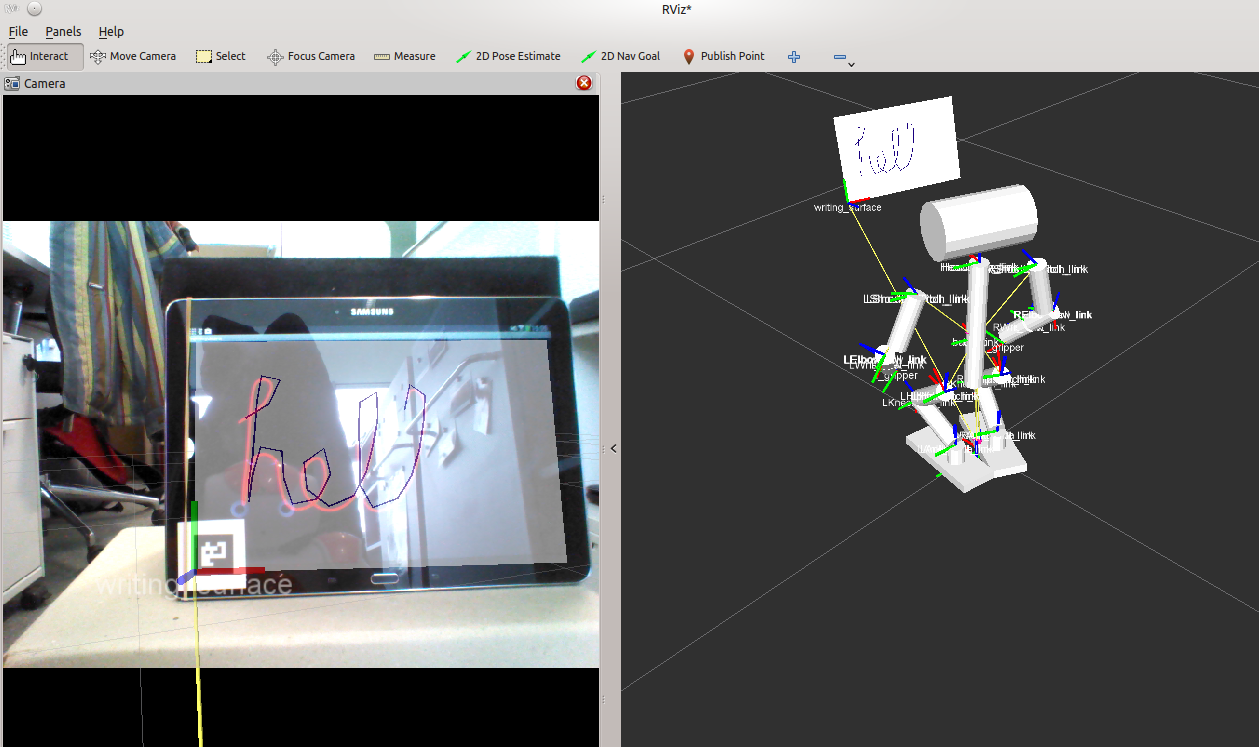
\includegraphics[width=0.45\textwidth]{figures/chilitagDetection_cameraOverlay.png}
    \caption[Detection of the tablet using a chilitag to represent the origin of
    the writing surface frame.]{\label{fig:tabletDetection}Detection of the
    tablet using a chilitag to represent the origin of the writing surface frame
(left: robot's camera image, with markers overlaid).}

\end{figure}% * <deanna.m.hood@gmail.com> 2014-09-04T11:21:59.328Z:
%
% this image is pretty bad, and doesn't add much
%


A demonstration of the robot executing a trajectory in synch with the tablet is
shown in Figure \ref{fig:naoWriting}\footnote{See
\url{https://www.youtube.com/watch?v=2qWFSJRxCU0} for a video of the
demonstration. }. % * <deanna.m.hood@gmail.com> 2014-09-04T11:40:30.176Z:
%
% this sounds dumb on paper.....
%


\subsection{Integration into a Robotic Handwriting Learning Agent}

The fusion of the embodied handwriting agent developed with the handwriting
learning algorithm presented in Section \ref{sec:learningAlgorithm} involves the
integration of three components. The robot and Android tablet application
present the writing process/result to the user, as in Section
\ref{sec:tabletSynch}. Furthermore, the tablet application is extended to act as
the primary medium for capturing user interaction, and publishes the user's
demonstrations when user is satisfied with their writing. The user
demonstrations are received by an interaction controller, running on a desktop
computer. It is responsible for getting the Nao to prompt and respond
appropriately to feedback received using a finite state machine to manage the
interaction stage. It also manages the learning algorithm, by inferring the
letter which user demonstrations are for, based on their position on the tablet,
and publish the shapes to be written which are generated by the learning
algorithm in response to the feedback.  


%Feedback from the user is passed to the controller with the location on the
%tablet that it occurred at, and the task of interpreting the shape which the
%feedback was intended for is left to the controller as it is aware of the
%location of published shapes. The appropriate response in terms of the learning
%algorithm is then taken for the respective shape. 

%%%%%%%%%%%%%%%%%%%%%%%%%%%%%%%%%%%%%%%%%%%%%%%%%%%%%%%%%%%%%%%%%%%%%%%%%%%%%%%%

%%%%%%%%%%%%%%%%%%%%%%%%%%%%%%%%%%%%%%%%%%%%%%%%%%%%%%%%%%%%%%%%%%%%%%%%%%%%%%%%

\section{A Tool for Social and Pedagogical Investigations} \label{sec:experiment}
\label{sec4}

In addition to constituting a technically novel system, the teachable robotic
agent presented represents a tool which may be used for investigating social and
pedagogical research questions. One such question that is being worked towards
is what impact to the outcomes of a handwriting intervention the addition of
such a teachable robotic agent would have. 

%\subsection{Interaction Context}

The interaction context which has been developed as a framework for addressing
such questions is one where participants are asked to improve the robot's
handwriting by correcting its letters. Figure~\ref{fig:pilotInteraction}
illustrates an example interaction sequence between the participant and the
robot, which consists of the following stages.

\begin{enumerate}

    \item The participant shows the robot one of five different 3-letter words
        to write, which, combined, consist of 7 different letters (`c', `e',
        `n', `o', `s', `u', `w'). Fiducial markers placed on the word cards to
        allow for detection with a camera. 

    \item The robot responds to the word request verbally and writes the letters
        by pointing at the tablet - placed in front of it with a vertical
        orientation - and imitating tracing the letters as they appear
        simultaneously by being displayed by the tablet. 

    \item The robot asks for feedback from the participant and they demonstrate
        how to write the letter which they feel needs to be corrected. The
        demonstration is performed by drawing on the tablet with a stylus,
        either with the tablet still in a vertical orientation or by unfolding
        the stand and laying the tablet flat on the desk. The position of the
        participant's demonstration on the tablet encodes the shape letter that
        it is a demonstration for. The participant can clear their shapes if
        they are unhappy with them or they are in the wrong position. When the
        button to signal that it is the robot's turn is pressed, the
        demonstration is sent to the controller.

    \item The interaction iterates, with participants taking turns to interact
        with the robot.

\end{enumerate}

%To allow the system to take input from the user on which words to draw,
%fiducial markers were placed on cards which were detectable by a
%previously-developed ROS node processing a camera stream. A node which
%processed the fiducial markers detected was then created to convert the card
%detected into an appropriate message for the controller. 
	
\begin{figure}[thpb!]
     \begin{center}
%
        \subfigure[The user shows a card to the robot with a word to write.]{%
            \label{fig:first}
            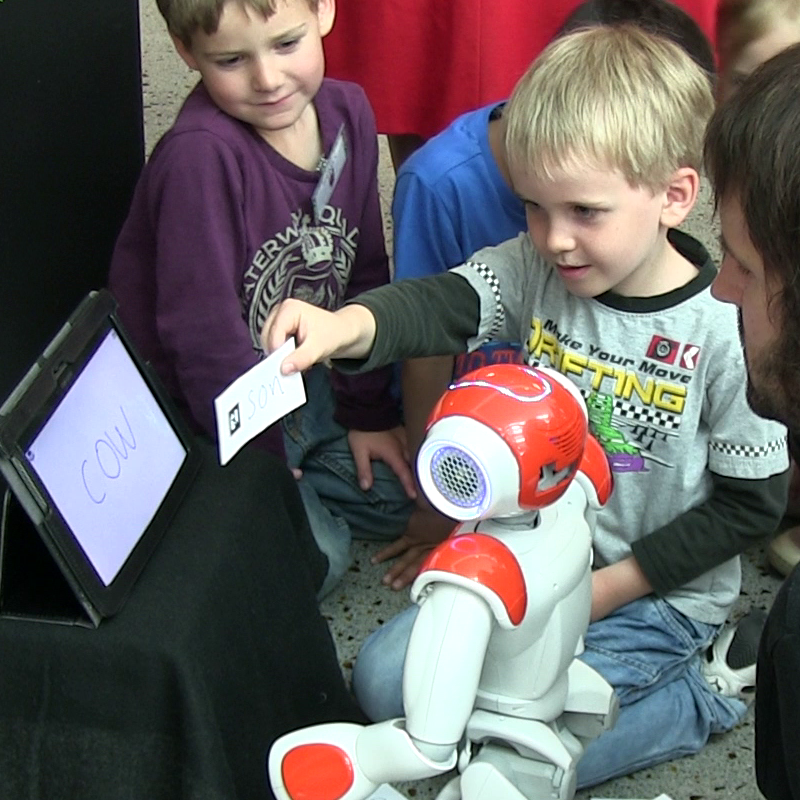
\includegraphics[width=0.2\textwidth]{figures/1card.png}
        }~
        \subfigure[The robot writes the word seen on the card and asks for feedback.]{%
           \label{fig:second}
           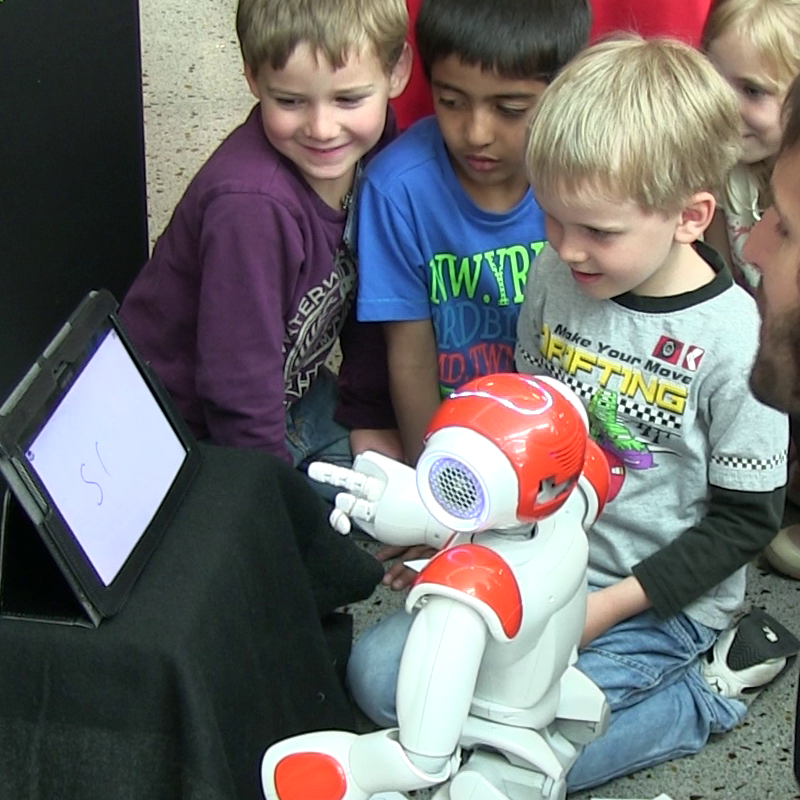
\includegraphics[width=0.2\textwidth]{figures/2word.png}
        }\\ %  ------- End of the first row ----------------------%
        \subfigure[The user provides feedback on the letters written via demonstration.]{%
            \label{fig:third}
            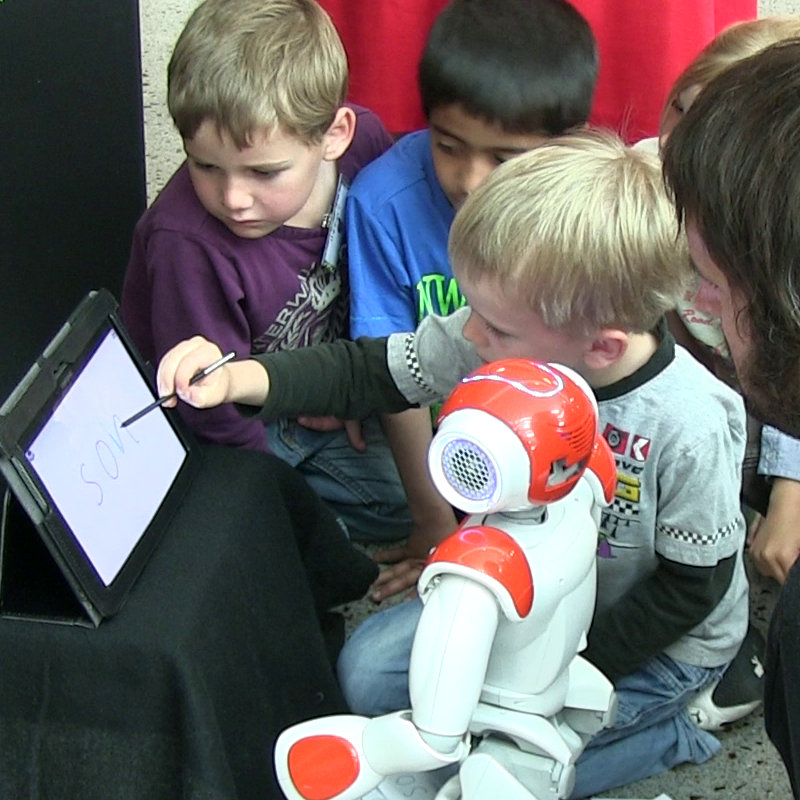
\includegraphics[width=0.2\textwidth]{figures/4correct.png}
        }~
        \subfigure[The robot responds to the feedback and asks for more.]{%
            \label{fig:fourth}
            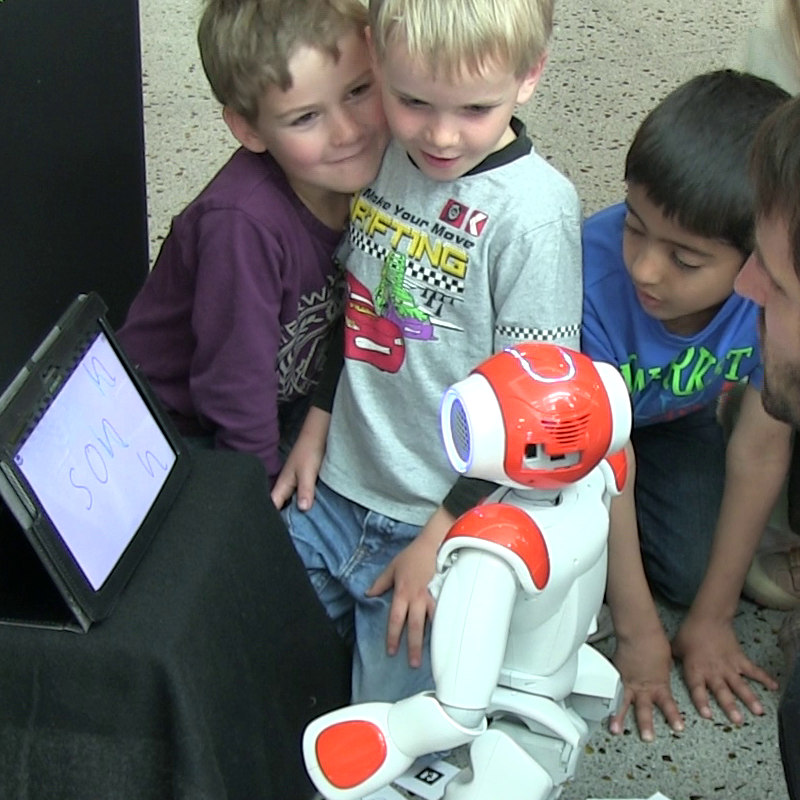
\includegraphics[width=0.2\textwidth]{figures/5iterateAsk.png}
        }%
%
    \end{center}
    \caption{%
        A user interacting with the robot in the learning by teaching interaction using demonstrations.
     }%
   \label{fig:pilotInteraction}
\end{figure}

%\subsection{Outcomes}

A pilot study has been conducted to evaluate the interaction in preparation for
an experiment to be conducted on the 10th-11th of June, 2014. The pilot study
consisted of four groups of approximately 8 children, aged 6-7 years. Outcomes
from the pilot study include information on how children interact with the
system, sample letters written by children, opinions from the teachers involved,
and insight into what experimental conditions might be appropriate for the
experiment. 

The system was validated, in that the learning algorithm and robotic writing
were believed by the children, and that the system withstood the interaction for
a total of 65 minutes, with the robot writing 96 letters, 49 of which in
response to demonstrations from the children, during that time. 

Another key point which came from the pilot study is that children were observed
giving advice to the child designated as the letter demonstrator, potentially
giving rise to the higher level paradigm of learning by \emph{teaching to
teach}. 

%\begin{itemize}
%
%\item Children would not intuitively write over the robot's letters, but rather
%above them. When instructed to write over the robot's letter, some participants
%would trace the letter as it had previously appeared as their demonstration. As
%such, the requested demonstration positioning will be modified for the
%experiment.
%
%\item While children spoke to the robot each time it requested feedback -
%suggesting that the anthropomorphised the robot - they also laughed when it
%wrote letters which were incorrect, which may suggest that they had not
%developed an empathetic connection with the robot by that point. 
%
%\item Children were observed giving advice to the child designated as the
%letter demonstrator, potentially giving rise to the higher level paradigm of
%learning by teaching to teach. 
%
%\end{itemize}

As a consequence of this observation, the upcoming experiment will address the
effect of the number of children interacting with the robot in order to
investigate the potential of the system to not only be used to set the context
of children tutoring the robot, but also children interacting as peer tutors
with each other.


Further research may discover how to best model/limit the learning speed of the
robot so that it is noticeably learning while not improving so fast as to limit
the long-term interaction potential for the system, which may turn out to be
child-dependent.

%\section{ADDITIONAL REQUIREMENTS}

\paragraph{Role of the experimenter}

%%%%%%%%%%%%%%%%%%%%%%%%%%%%%%%%%%%%%%%%%%%%%%%%%%%%%%%%%%%%%%%%%%%%%%%%%%%%%%%%
\section{Conclusions and Future Work}

%\subsection{Conclusions}

The technical challenges involved in developing a teachable robotic agent in the
context of handwriting which have been addressed in this work include:

\begin{itemize}

    \item developing capabilities for a robot with limited fine motor
        capabilities, such as the Nao, to engage in the act of handwriting in a
        way that is believable for interacting with children, which has been
        accomplished by leveraging simulated handwriting with a synchronised
        tablet;

    \item developing a system for generating poorly written letters appropriate
        for simulating a na\"ive learner in the context of handwriting, achieved
        by using statistical shape models through PCA of observations of the
        trajectory of the same letter;

    \item developing an algorithm capable of incorporating user feedback and
        demonstrations in order to adapt the generated handwriting quality so as
        to simulate a teachable agent, which has been implemented by maintaining
        a learning algorithm in the parameter space of the shape models and
        converging towards the parameters of user demonstrations; and

    \item integrating the system into a working interaction suitable for
        engaging children in the learning by teaching paradigm, accomplished by
        fusing the robotic drawing capabilities and the learning algorithm for
        handwritten letters established.

\end{itemize}

%By leveraging the technology of a wirelessly synchronised tablet displaying a
%writing trajectory, the requirements for a robot with limited fine motor
%capabilities to accurately manipulate a writing implement have been reduced to
%instead requiring that the robot roughly trace the trajectory as it is
%simultaneously displayed on the tablet. Thus, capabilities for the Nao to
%engage in simulated handwriting have been demonstrated. By further lifting the
%constraint that the robot must draw with a writing instrument and allowing it
%instead to draw with its finger, in addition to increasing the range of
%trajectories which the robot is able to reach, the necessary accuracy in the
%robot's trajectory following is reduced as it is not necessary for the finger
%to physically touch the writing surface at the trajectory position for the
%simulation to be believable. As the motion control is currently limited to the
%position of the robot's hand rather than the writing tip, the reduced need for
%accurate motion in order to have a believable simulation was leveraged upon in
%the presented system to produce results with the robot drawing with its finger
%of sufficient accuracy. 

%Statistical shape modeling using principal component analysis on a dataset of
%writing trajectories for a letter has been employed to generate shape models of
%different letters/allographs. These models, generated through unsupervised
%methods, have been shown to capture the internal proportions of letters in a
%similar way to how human intuition would identify the possible shape variances
%(width/height/proportional size of loops, skewness, etc.). As a result, the
%models have been used to generate synthetic letters which yield shapes
%appropriate for use in an artificial intelligence algorithm which uses user
%feedback on the best letter from a set of candidates drawn to converge to the
%parameter values of the selected shapes after some iterations.

%The letter model has been used to determine the parameter values of shapes
%demonstrated by the user. Provided that the user demonstrates the shape in the
%same style as those used to generate the shape model (i.e., with the strokes in
%the appropriate order and direction), the parameters of the demonstration may
%then be used as input to the learning algorithm to converge towards the user's
%writing demonstrations. 

%The fusion of the robotic drawing capabilities and the learning algorithm for
%handwritten letters has resulted in a teachable robotic agent which can engage
%users in the learning by teaching paradigm in the context of handwriting. As
%such, the system developed has been shown to accomplish the technical goals
%which were set out to be achieved, and the implications of such a system
%evaluation of the system is underway, with an in situ interaction with primary
%school students being conducted in the coming weeks. 

\subsection{Why a robot?}



\subsection{Future Work}

In the scope of open technical questions, it remains to be seen how shape models
for letters might be generated which capture the full range of mistakes typical
of children learning handwriting: extending the current system capable of
incorporating internal proportion and global deformation errors to one which can
also generate missing subparts of the letter, or break the letter down into
primitive strokes at will, for example. While we expect that incorporating a
database of letters drawn by children into the shape modeling process would
facilitate this, the current system has conceptual (a PCA only approach can not
generate or learn a different shape topology) and technical (no support for
multi-stroke shapes) limitations that need to be overcome.

In terms of the interaction experience, the current experimental setting, while
technically autonomous, can not robustly recover from situations outside of the
nominal protocol (presented in section~\ref{sec4}), and consequently still requires the
presence of an experimenter. The robot state machine would require to be
extended in non-trivial ways to allow for long, fully autonomous, interactions
with children.

%it may be interesting to investigate
%which other technology could be incorporated into the system for a more fluid
%interaction, such as integrating the user's gaze information to infer when the
%user is finished with a demonstration, or using a classification algorithm to
%determine which letter has been demonstrated irrespective of its positioning.

On the educational side, open questions include how the handwriting error
generation of the system may be abstracted to a higher level of control so that
a teacher may configure it to work with a child on a particular type of
mistakes, based on the child's performance. Where would the balance lie between
developing autonomous capabilities for the system to determine the child's
difficulties, and empowering the teaching staff to decide for themselves
instead? And, as a result, the ultimate question for this area of research is
to address what impact to the outcomes of a long-term handwriting intervention the
addition of such a teachable robotic agent would have: does it impact the
motivation of the participants, their self-esteem, and/or the learning gains
that they experience? We are currently considering running a long-term study
(about 20 hours of interactions per child) that would provide better evidences
to answer these questions.

\subsection{Impact and Conclusion}

We believe this article introduces three noteworthy contributions: an innovative
application of data processing and artificial intelligence for the generation and
learning of hand-written letters suitable for educative purposes; a robotic
system that has been experimentally proven to provide convincing scaffolding for
complex human-robot interactions (teacher-learner social interactions, learning by
demonstration); an initial experimental investigation of what appears to be a
new role for robots in education.

Because it has the strongest impact for the human-robot interaction community,
we would like to develop this last point in particular. The work presented here
investigates a particular role for a robot in the education of handwriting: not
only the robot is actively performing the activity (it draws letters), but it
does so in a way that engages the child in a very specific social role. The child
is the teacher, the robot is the learner: the child must engage in a
(meta-)cognitive relation with the robot to try to understand why the
robot fails and how to help it best.  Here, the robot is not only an activity
facilitator or orchestrator: its physical presence and embodiment induce agency
and anthropomorphizing, and cognitively engage the child into the learning
activity, which we predict to lead to higher learning efficacy.

Also notable, the robot is not used in the usual context of robotics or computer
education, but instead in an activity -- handwriting -- that requires fine
physical skills. In such activities, the embodied nature of the robot makes a
lot of sense (due to motor mimicry, the arm motion for instance is, \emph{by
itself}, part of the teaching). Along those lines, we hope to see more research
on non-STEM educational applications of robotics.

Beyond handwriting, we believe that this work provides a novel perspective on
the role for robots in the education landscape. \emph{Learning by teaching} is a
powerful paradigm because not only its pedagogical efficacy is proven, but it
also positively impacts the child's motivation and self-esteem. We have
discovered that it is also a very relevant context of use for robots. Indeed,
when facing a child with school difficulties, robots can play a role (being the
``even more ignorant student'') that neither the adults nor the peers (because
of the social effects it would induce) can convincingly play.

The strong social impact of early school problems makes research in this field
a certainly useful challenge for HRI.

%%%%%%%%%%%%%%%%%%%%%%%%%%%%%%%%%%%%%%%%%%%%%%%%%%%%%%%%%%%%%%%%%%%%%%%%%%%%%%%%
%%\section{ACKNOWLEDGMENTS}

%The authors gratefully acknowledge the contribution of National Research Organization and reviewers' comments.


%%%%%%%%%%%%%%%%%%%%%%%%%%%%%%%%%%%%%%%%%%%%%%%%%%%%%%%%%%%%%%%%%%%%%%%%%%%%%%%%

%\begin{thebibliography}
\bibliographystyle{abbrv}
\bibliography{library}

%\end{thebibliography}

\end{document}
